
%(BEGIN_QUESTION)
% Copyright 2010, Tony R. Kuphaldt, released under the Creative Commons Attribution License (v 1.0)
% This means you may do almost anything with this work of mine, so long as you give me proper credit

A coke {\it calcining} operation (where petroleum coke is burned to decrease its hydrogen content) uses a large bin to collect coke dust that forms around its hooded conveyor systems.  The level of coke dust inside this bin is measured by a gamma-radiation instrument:

$$\includegraphics[width=15.5cm]{i00320x01.eps}$$

Explain how this system uses nuclear radiation to measure coke dust level.

\vskip 20pt \vbox{\hrule \hbox{\strut \vrule{} {\bf Suggestions for Socratic discussion} \vrule} \hrule}

\begin{itemize}
\item{} Why does this system use multiple radioactive sources?  Why do you suppose one is not sufficient?
\item{} Suppose some radioactive material accidently entered the storage bin along with coke dust.  Would this shift the level instrument's {\it zero}, the {\it span}, or both?
\item{} Identify some alternative technologies which we could use to measure the coke dust level.
\item{} What function does a {\it cyclone separator} perform, based on an analysis of this simple process flow diagram?  Note: cyclone separators are commonly used in sawmill operations, to handle wood chips in a moving air stream.
\end{itemize}

\underbar{file i00320}
%(END_QUESTION)





%(BEGIN_ANSWER)

%(END_ANSWER)





%(BEGIN_NOTES)

Any substance placed in the path of nuclear radiation will attenuate that radiation to some extent, the amount of attenuation dependent upon the radiation path length and the material's density.

\vskip 10pt

Safety issues:

\begin{itemize}
\item{} How to ``shut off'' the radiation source
\item{} Making sure the source is aimed the correct way
\item{} Limiting personal exposure time to the radiation pathway
\item{} Maintaining safe distances to leverage the {\it inverse square law} of radiation
\end{itemize}


%INDEX% Measurement, level: radiation (nuclear)
%INDEX% Process: coke dust storage tank level

%(END_NOTES)


